\begin{flushleft}


Meie eesmärgiks on kujutada keha liikumist graafilisel tasapinnal. Kuna me kujutame liikumist tasapinnal, siis meil on keha asukoha määramiseks vaja kahte argumenti. Esimene neist peab meile ütlema keha horisontaalset asukohta (ehk kui vasakul või paremal ta asub), ning teine määrab vertikaalse asukoha (ehk kui kõrgel või madalal keha tasapinnal asub). 


Kasutame selle jaoks traditsioonilist Descartesi koordinaatsüsteemi.

\begin{figure}[h]  
\centering 
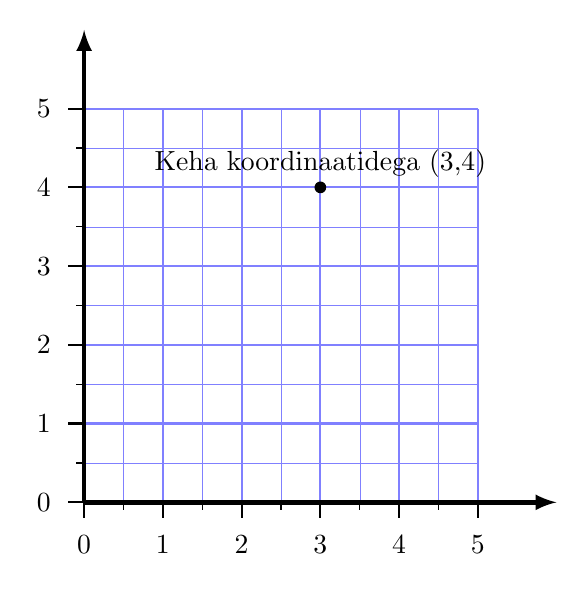
\begin{tikzpicture}
% Draw the grid
\tikzset{help lines/.style={color=blue!50}}
\draw[thick,step=1cm,help lines] (0,0) grid (5,5);
\draw[ultra thin,step=.5cm,help lines] (0,0) grid (5,5);
% Draw axes
\draw[ultra thick,-latex] (0,0) -- (6,0);
\draw[ultra thick,-latex] (0,0) -- (0,6);
% the co-ordinates -- major
\foreach \x in {0,1,...,5} {     % for x-axis
\draw [thick] (\x,0) -- (\x,-0.2);
}
\foreach \y in {0,1,...,5} {   %% for y-axis
\draw [thick] (0,\y) -- (-0.2,\y);
}
% the numbers
\foreach \x in {0,1,...,5} { \node [anchor=north] at (\x,-0.3) {\x}; }
\foreach \y in {0,1,...,5} { \node [anchor=east] at (-0.3,\y) {\y}; }
% the co-ordinates -- minor
\foreach \x in {.5,1.5,...,4.5} {
\draw [thin] (\x,0) -- (\x,-0.1);
}
\foreach \y in {.5,1.5,...,4.5} {
\draw [thin] (0,\y) -- (-0.1,\y);
}
\node at (3,4) [circle, fill, inner sep=1.5pt] {};
\node at (3,4)[anchor=south] {Keha koordinaatidega (3,4)};
\end{tikzpicture}
\caption{Keha asukoht tasapinnal}
\label{Joonis 1}
\end{figure}


Selline pilt kirjeldaks vaid ühte instantsi/iteratsiooni ehk ajahetke.
Selleks, et kujutada liikumist samal pinnal, tuleb meil joonist iga iteratsiooni/ajahetke järel uuendada.

Näiteks kui kujutada lineaarset liikumist, mis on määratud funktsiooniga $y=x+1$, kus $x$ määrabki ajahetke, ning keha algne asukoht on punktis $(1,2)$, siis saaksime järgmise kolme ajahetke jaoks kolm järgmist kaadrit:

\begin{figure}[h]  
\centering 

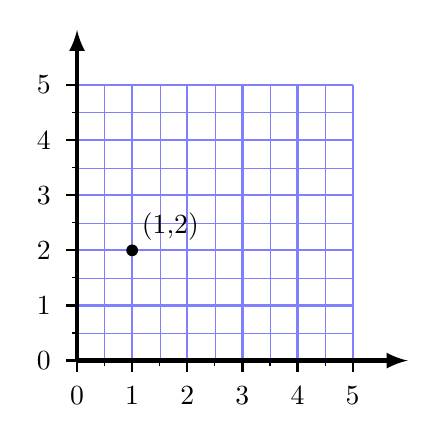
\begin{tikzpicture}[scale=0.7]
     % Draw the grid
\tikzset{help lines/.style={color=blue!50}}
\draw[thick,step=1cm,help lines] (0,0) grid (5,5);
\draw[ultra thin,step=.5cm,help lines] (0,0) grid (5,5);
% Draw axes
\draw[ultra thick,-latex] (0,0) -- (6,0);
\draw[ultra thick,-latex] (0,0) -- (0,6);
% the co-ordinates -- major
\foreach \x in {0,1,...,5} {     % for x-axis
\draw [thick] (\x,0) -- (\x,-0.2);
}
\foreach \y in {0,1,...,5} {   %% for y-axis
\draw [thick] (0,\y) -- (-0.2,\y);
}
% the numbers
\foreach \x in {0,1,...,5} { \node [anchor=north] at (\x,-0.3) {\x}; }
\foreach \y in {0,1,...,5} { \node [anchor=east] at (-0.3,\y) {\y}; }
% the co-ordinates -- minor
\foreach \x in {.5,1.5,...,4.5} {
\draw [thin] (\x,0) -- (\x,-0.1);
}
\foreach \y in {.5,1.5,...,4.5} {
\draw [thin] (0,\y) -- (-0.1,\y);
}
\node at (1,2) [circle, fill, inner sep=1.5pt] {};
\node at (1,2)[anchor=south west] {(1,2)};
\end{tikzpicture}% NO EMPTY LINE HERE!!!! 
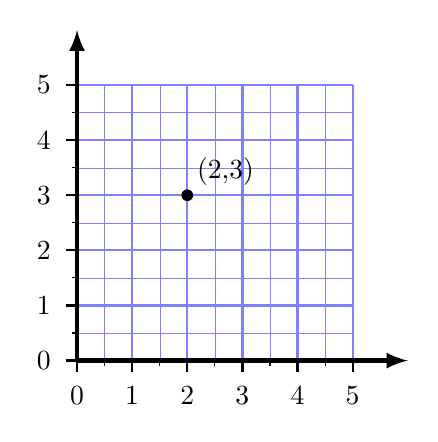
\begin{tikzpicture}[scale=0.7]  
     % Draw the grid
\tikzset{help lines/.style={color=blue!50}}
\draw[thick,step=1cm,help lines] (0,0) grid (5,5);
\draw[ultra thin,step=.5cm,help lines] (0,0) grid (5,5);
% Draw axes
\draw[ultra thick,-latex] (0,0) -- (6,0);
\draw[ultra thick,-latex] (0,0) -- (0,6);
% the co-ordinates -- major
\foreach \x in {0,1,...,5} {     % for x-axis
\draw [thick] (\x,0) -- (\x,-0.2);
}
\foreach \y in {0,1,...,5} {   %% for y-axis
\draw [thick] (0,\y) -- (-0.2,\y);
}
% the numbers
\foreach \x in {0,1,...,5} { \node [anchor=north] at (\x,-0.3) {\x}; }
\foreach \y in {0,1,...,5} { \node [anchor=east] at (-0.3,\y) {\y}; }
% the co-ordinates -- minor
\foreach \x in {.5,1.5,...,4.5} {
\draw [thin] (\x,0) -- (\x,-0.1);
}
\foreach \y in {.5,1.5,...,4.5} {
\draw [thin] (0,\y) -- (-0.1,\y);
}
\node at (2,3) [circle, fill, inner sep=1.5pt] {};
\node at (2,3)[anchor=south west] {(2,3)};
\end{tikzpicture}
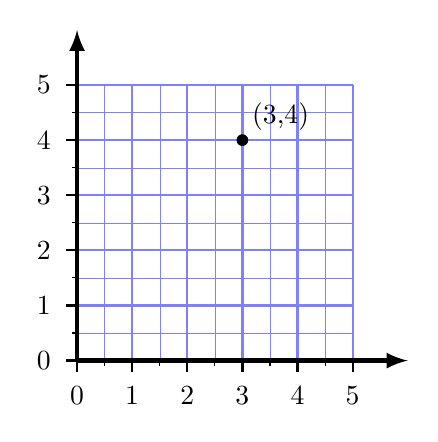
\begin{tikzpicture}[scale=0.7]
     % Draw the grid
\tikzset{help lines/.style={color=blue!50}}
\draw[thick,step=1cm,help lines] (0,0) grid (5,5);
\draw[ultra thin,step=.5cm,help lines] (0,0) grid (5,5);
% Draw axes
\draw[ultra thick,-latex] (0,0) -- (6,0);
\draw[ultra thick,-latex] (0,0) -- (0,6);
% the co-ordinates -- major
\foreach \x in {0,1,...,5} {     % for x-axis
\draw [thick] (\x,0) -- (\x,-0.2);
}
\foreach \y in {0,1,...,5} {   %% for y-axis
\draw [thick] (0,\y) -- (-0.2,\y);
}
% the numbers
\foreach \x in {0,1,...,5} { \node [anchor=north] at (\x,-0.3) {\x}; }
\foreach \y in {0,1,...,5} { \node [anchor=east] at (-0.3,\y) {\y}; }
% the co-ordinates -- minor
\foreach \x in {.5,1.5,...,4.5} {
\draw [thin] (\x,0) -- (\x,-0.1);
}
\foreach \y in {.5,1.5,...,4.5} {
\draw [thin] (0,\y) -- (-0.1,\y);
}
\node at (3,4) [circle, fill, inner sep=1.5pt] {};
\node at (3,4)[anchor=south west] {(3,4)};
\end{tikzpicture} 
\caption{Vasakul: Keha asukoht algsel ajahetkel. Keskel: Keha asukoht teisel ajahetkel. Paremal: Keha asukoht viimasel ajahetkel.} \label{Joonis 2}  
\end{figure}

Ehk vaatleja ekraanil näeks liikumine välja nagu (Joonis \ref{Joonis 3}).
\vspace{2mm}

\begin{figure}[h]
\centering
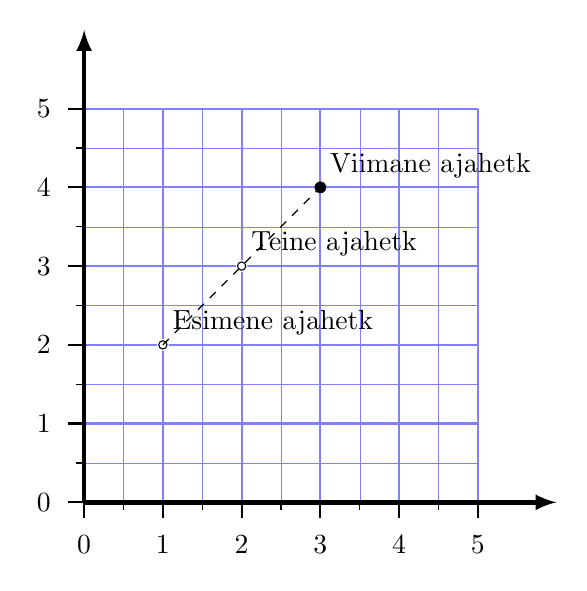
\begin{tikzpicture}
     % Draw the grid
\tikzset{help lines/.style={color=blue!50}}
\draw[thick,step=1cm,help lines] (0,0) grid (5,5);
\draw[ultra thin,step=.5cm,help lines] (0,0) grid (5,5);
% Draw axes
\draw[ultra thick,-latex] (0,0) -- (6,0);
\draw[ultra thick,-latex] (0,0) -- (0,6);
% the co-ordinates -- major
\foreach \x in {0,1,...,5} {     % for x-axis
\draw [thick] (\x,0) -- (\x,-0.2);
}
\foreach \y in {0,1,...,5} {   %% for y-axis
\draw [thick] (0,\y) -- (-0.2,\y);
}
% the numbers
\foreach \x in {0,1,...,5} { \node [anchor=north] at (\x,-0.3) {\x}; }
\foreach \y in {0,1,...,5} { \node [anchor=east] at (-0.3,\y) {\y}; }
% the co-ordinates -- minor
\foreach \x in {.5,1.5,...,4.5} {
\draw [thin] (\x,0) -- (\x,-0.1);
}
\foreach \y in {.5,1.5,...,4.5} {
\draw [thin] (0,\y) -- (-0.1,\y);
}
\node at (3,4) [circle, fill, inner sep=1.5pt] {};
\node at (3,4)[anchor=south west] {Viimane ajahetk};

\node at (2,3) [circle, fill=white, inner sep=1.5pt] {};
\node at (2,3)[anchor=south west] {Teine ajahetk};
\draw (2,3) circle (1.5pt);

\node at (1,2) [circle, fill=white, inner sep=1.5pt] {};
\node at (1,2)[anchor=south west] {Esimene ajahetk};
\draw (1,2) circle (1.5pt);
\draw[dashed] (1,2)--(3,4);
\end{tikzpicture}
\caption{Keha liikumine tasapinnal}
\label{Joonis 3}
\end{figure}

\vspace{2mm}
On näha, et keha justkui hüppaks punktist $(1,2)$ punkti $(2,3)$ ning viimaks ka punkti $(3,4)$. Ehk teisisõnu, see ei näe eriti liikumise moodi välja. Kahjuks ei saa reaalset liikumist ekraanil kujutada ning me peamegi piirduma selliste ''hüppetega'' punktist punkti. Küll aga on meil võimalus inimese silma natuke petta. Kui me vähendaksime ajahetkede vahemike, siis väheneksid ka ''hüppete'' vahemikud ja seega näeks liikumine märkimisväärselt sujuvam välja \cite{fpsyoutube}.

\vspace{2mm}
Kuid ajahetkede vahemike me lõputult väikseks teha ka ei saa, kuna sellisel juhul oleks arvuti sunnitud rohkem ja seega kauem arvutusi teostama.

\vspace{2mm}
Väidetavalt \cite{potter2014detecting} suudab inimese silm kujutist tuvastada 13 millisekundiga. Oma rakenduste loomisel, võikski sellise ajavahemikuga piirduda. Väiksema ajavahemiku valimine meie kujutise näivat liikumist ei täiustaks, kuna inimese silm ei jõuaks nii kui nii sellega järge pidada.

\vspace{2mm}
Meie rakenduste esimestel katsetel, proovime liikumisi arvutada 13 millisekundiliste ajahetkedega. Kui säärane ajavahemik osutub arvuti jaoks ülejõu käivaks, siis suurendame ajahetkede vahemike sammuga 13, seni kuni saavutame piisavalt sobiva tulemuse.


\end{flushleft}